\subsection{Reactive Programming}

\textbf{Reactive programming} is a paradigm built around the notions of
\textit{continuous time-varying values} and \textit{propagation of change},
ideal for the development of event-driven applications
\cite{ReactiveProgramming}. In particular, computation is expressed in terms of
dependencies between flows of information, so that when some information
changes, all the dependent information is updated automatically by the
underlying execution model.

Consider the following program for computing the sum of two variables.

\begin{lstlisting}
  var1 = 1
  var2 = 2
  var3 = var1 + var2  # var3: 3
  var1 = 3            # var3: 5
  var2 = 1            # var3: 4
\end{lstlisting}

In reactive programming, the program is translated into a \textbf{computational
graph} (shown in Figure \ref{figure:dependency-graph}), expressing the
dependencies of the variable \texttt{var3} on the variables \texttt{var1} and
\texttt{var2}, so that any future reassignment of \texttt{var1} or
\texttt{var2} will be automatically reflected on the value of \texttt{var3},
unlike standard imperative programming. Due to their non-standard behavior,
variables in reactive programming are also called \textbf{reactive variables}.

\begin{figure}[h]
  \centering
  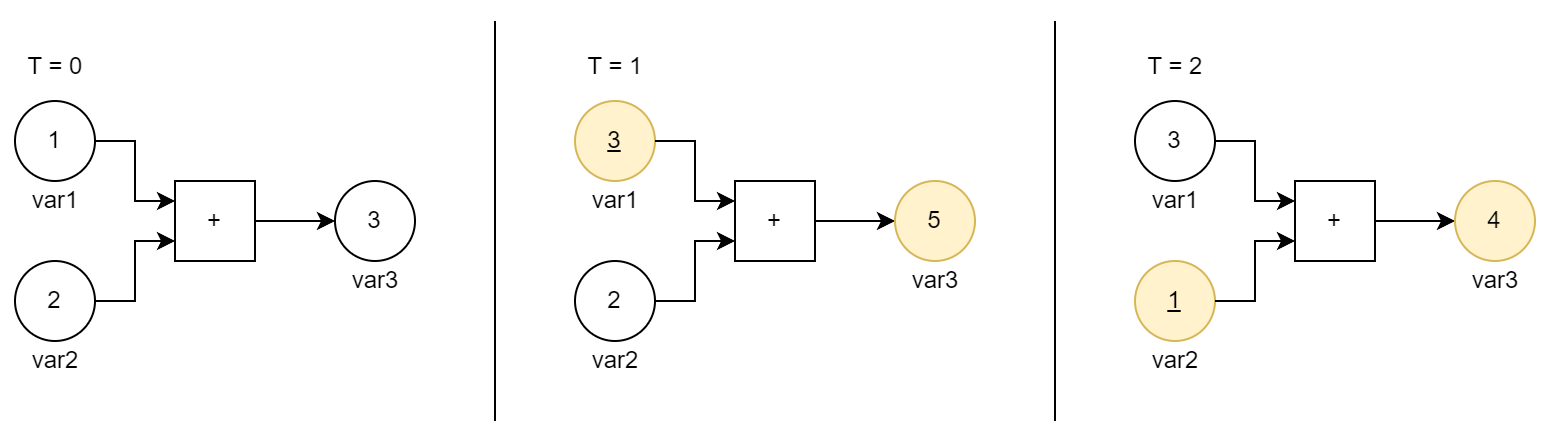
\includegraphics[width=\textwidth]{resources/figures/dependency-graph.png}
  \caption{
    A computational graph in reactive programming: nodes (circles) represents
    reactive variables and their current values; yellow nodes represent a
    propagation of change; underlined yellow nodes represent the
    start of a propagation of change; operations (squares) represent a type
    of dependency between nodes (when the type of dependency is not relevant,
    they may be omitted). For example, at time \texttt{T=1}, \texttt{var1} was
    reassigned to value 3, triggering an update of \texttt{var3} to value 5.
  }
  \label{figure:dependency-graph}
\end{figure}

A value assigned to a reactive variable can be either a \textbf{behavior}, that
is a time-varying value in continuous time (e.g. time itself), or an
\textbf{event stream}, that is a potentially infinite sequence of events,
occurring at discrete points in time (e.g. mouse clicks). Generally, behaviors
are used to model time-varying states, which can always be sampled, while event
streams are used to model state updates, which exist only in the discrete point
in time when they are triggered. However, some implementations of reactive
programming avoid such distinctions.

In order to be applied to reactive variables, standard operators should be
transformed into \textit{reactive operators}. Such transformation is called
\textbf{lifting} and requires changing the type signature of the operators and
properly updating the computational graph. The semantics of reactive
programming languages change depending on how lifting is implemented:
\textit{implicit lifting} allows to apply standard operators to reactive
variable as-is (transforming them under the hood); \textit{explicit lifting}
provides a \textbf{lift} primitive to apply the transformation to a standard
operator; \textit{manual lifting} does not implement lifting, requiring the
developer to manually sample and compose the values of behaviors.

Reactive operators are used to build the computational graph of a reactive
program, creating dependencies between reactive variables. Some reactive
programming implementations enjoy the property of \textbf{multidirectionality},
allowing the definition of bidirectional dependencies or cyclic graphs. Some
may support \textbf{switching}, allowing the definition of dynamic
computational graphs whose dependencies change over time.

The \textbf{evaluation model} of a reactive programming language deals with the
propagation of changes within a computational graph. Propagation of change
always involves a \textbf{producer} to trigger the change (e.g. a dependency)
and a \textbf{consumer} to react to the change (e.g. a dependent). The
evaluation model can be categorized based on the roles of the two entities:
\begin{itemize}
  \item \textbf{Pull-Based}: consumers poll producers for their events,
        resulting in \textit{lazy reaction} (\textit{demand-driven propagation}),
        as polling may happen after the time when the events were fired at the
        discretion of the consumer. This approach works best with time-varying
        values in continuous time.
  \item \textbf{Push-Based}: producers push events to the consumers, resulting
        in \textit{eager reaction} (\textit{data-driven propagation}), as state
        changes are propagated as they are produced. This approach works best
        when instantaneous reactions are a requirement.
\end{itemize}

While the push-based evaluation model is adopted in most recent implementations
of reactive programming, it requires additional mechanisms to avoid
\textbf{glitches}, which are inconsistent events, generated when a dependent is
updated before all of its dependencies are up-to-date, resulting in a
combination of new and stale events. Consider the following example.

\begin{lstlisting}
  var1 = 1
  var2 = var1 * 1     # var2: 1
  var3 = var1 + var2  # var3: 2
  var1 = 2            # var3: 3 (glitch); var2: 2; var3: 4 (correct)
\end{lstlisting}

In the example, when \texttt{var1} is reassigned (line 4), the propagation of
change may reach \texttt{var3} before \texttt{var2}, leading to an inconsistent
value for \texttt{var3}, since \texttt{var2} is not up-to-date. Eventually,
\texttt{var2} will also be updated and so \texttt{var3} will reach a consistent
value. However, any dependency on \texttt{var3} would have already suffered
from its inconsistencies (e.g. incorrect program state, wasteful
recomputations), hence the requirement of mechanisms for \textbf{glitch
freedom}. Note that glitches are a consequence of inconsistent individual
handling of simultaneous events or reactions.

Most implementations of push-based reactive programming guarantee glitch
freedom in non-distributed environments. However, an important extension of
reactive programming is \textbf{distributed reactive programming}, which allows
expressing and managing the dependencies between the components of a
distributed system by distributing the nodes of a computational graph across
multiple machines (e.g. in "\texttt{var3 = var1 + var2}", \texttt{var1},
\texttt{var2} and \texttt{var3} may be located in different machines). Recent
progress shows that is possible to guarantee glitch freedom also in push-based
distributed reactive programming for acyclic graphs \cite{QPROP}, or at
different levels of consistency \cite{DREAM}, while retaining scalability and
parallelism.

Reactive programming is most suitable for designing event-driven applications,
achieving better declarativity and looser coupling between components with
respect to standard \textbf{event-driven programming} paradigms, such as the
\textit{observer} pattern\footnote{a pattern for event-driven programming, in
which consumers react to events by registering some callbacks
(\textit{listeners}) to the event producers, so that they may be executed each
time a new event is triggered. Callbacks may also trigger other events,
creating a dependency graph between callbacks. In fact, most reactive
implementations are an abstraction over this pattern.}. In fact, the former
hides how the propagation of change is implemented in the system, letting the
developer focus solely on the behavior of the program, while the latter
requires the developer to manually implement dependencies as events that may
trigger dependent events, resulting in a flow of control that is harder to
understand and nested transitive dependencies that are harder to detect.
